\section{Velocity Model of the Vehicle}
In this section the \textit{Vehicle} block in \chapref{cha:ModelOfVehicle} \figref{fig:StartTotalModelsystem} is opened up and modelled regarding the velocity of the vehicle. In \figref{fig:Velocitymodelplantopen} the opening of the \textit{Vehicle} block is illustrated.

\begin{figure}[H]
	\centering
	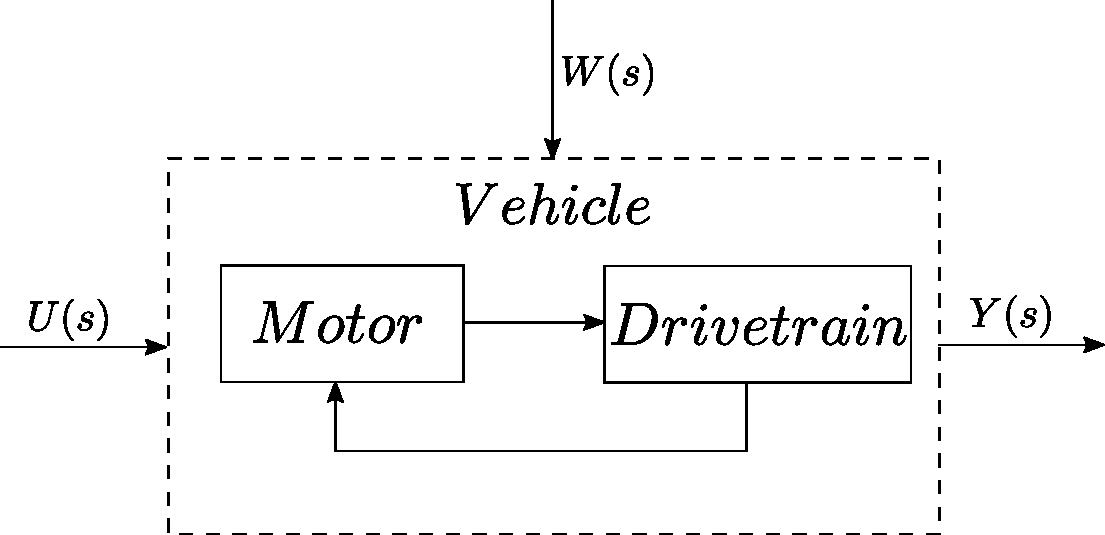
\includegraphics[scale=0.6]{figures/plantopen.pdf}
	\caption{The \textit{Vehicle} block in \chapref{cha:ModelOfVehicle} \figref{fig:StartTotalModelsystem} is opened up and illustrated in more detail}
	\label{fig:Velocitymodelplantopen}
\end{figure}

The velocity model of the \textit{vehicle} has been split up into a motor and a drivetrain section. The motor receives an input from the controller regulating its supplied voltage. the motor then delivers a rotational force as an output to the drivetrain. The drivetrain then generates the actual speed as the output of the \textit{Vehicle} block. as well as supplying the motor with an angular velocity which is dependent on the total inertia of the system, and thereby insures that the motor is affected by its load. The two sections, the motor and drivetrain, is generated by only considering the parameters affecting the vehicle when the vehicle is driving in a straight line. Thus, excluding the differential steering and thereby only modelling the system when the wheels have the exactly same velocity.

In the following subsection the motor will be modelled.